\section{Study 2: Understanding Explanations and Feedback with a High Quality Model}
%
In Study~1, expectations rose with feedback but not explanations and satisfaction fell with explanations but rose with feedback.
%
As the Study~1 model's low quality appeared to overwhelm participants' subjective ratings, an additional study had a higher quality model. While we expected participants to be more satisfied with the higher quality model (e.g., observed and stated model accuracy can affect users' trust~\cite{Yin2019UnderstandingModels}), we retained the Study~1 hypotheses regarding our primary measures (frustration and expected change).

\subsection{Method}
This experiment was exactly the same as Study~1 with the exceptions described here. We trained the \texttt{MultinomialNB} classifier on $200$ labeled training emails ($100$ from each class), with $94.4\%$ accuracy on the test set. This model predicted the correct label for $18$ of the $20$ emails in the interaction phase. As in Study~1, we chose four emails for the evaluation phase (two ``same'' and two ``similar''), but because of the higher accuracy of the model in Study~2 there were no available emails that were ``similar'' to ones the model labeled incorrectly in the evaluation phase; thus, both of the ``similar'' emails were similar to previously correct ones. 

As in Study~1, we recruited $180$ participants ($99$ female, $78$ male, $3$ unspecified). Two participants were aged 18--24 years old, 46 aged 25--34, 66 aged 35--44, 43 aged 45--54, 16 aged 55--64, and 6 aged 65--74. Participants had varied prior knowledge of machine learning (63 participants had none, 65 had a little, 50 had some, two had a lot, and none had expert), hockey (23 had none, 64 had a little, 58 had some, 25 had a lot, and none had expert), and baseball (12 had none, 37 had a little, 66 had some, 54 had a lot, and 11 had expert).

Study sessions took on average $22.8$ minutes ($SD=14.6$), and we used the same measures and data analyses as in Study~1. Our dataset included all 180 participants. We used the Study~1 codes to code the open-ended responses for frustration and expected change. We refer to participants as HP1--HP180.

\newcommand{\FigureHighMeasure}{
\begin{figure}[t]
    \centering
    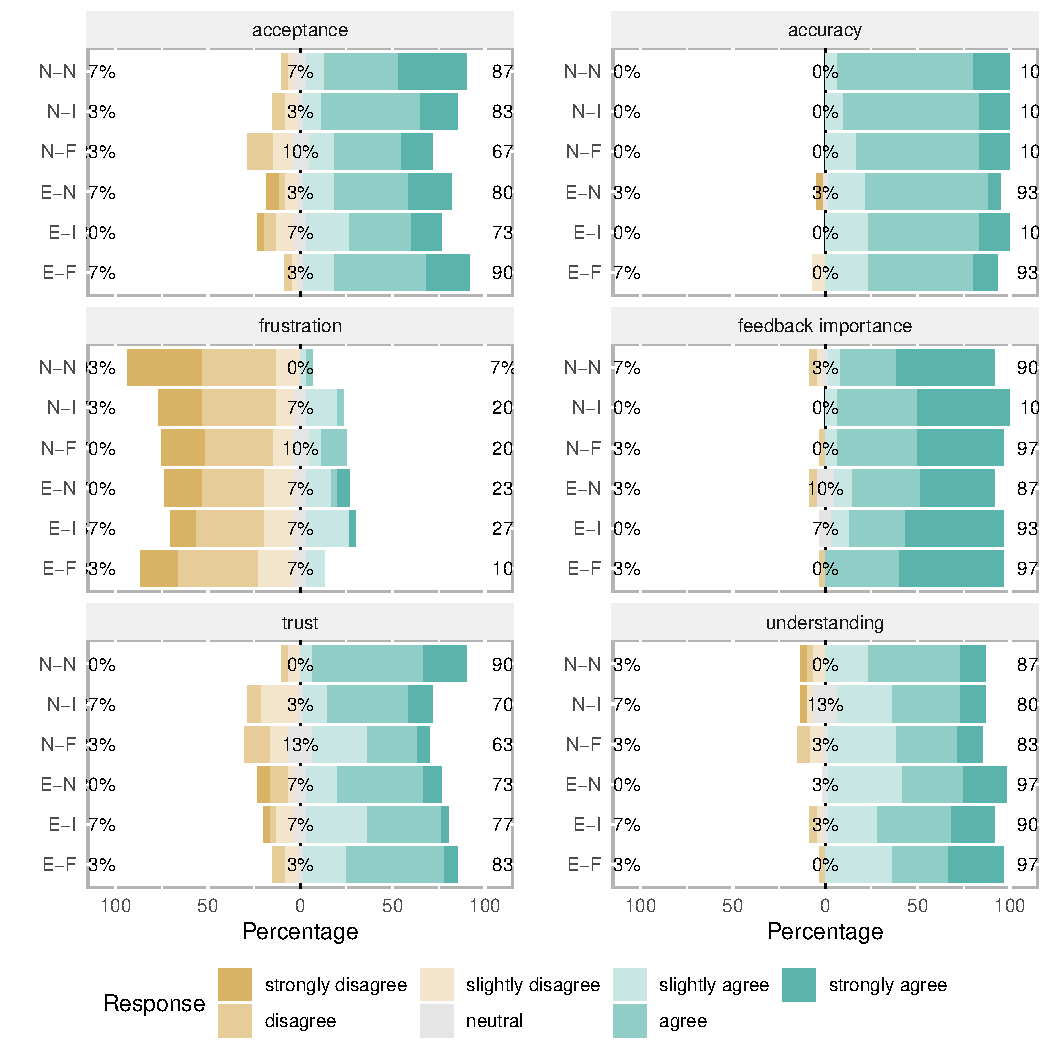
\includegraphics[width=.48\textwidth]{figures/study2-measures.pdf}
    \caption{Study 2 responses by condition for the main subjective measures (except expected change). Participants were more satisfied, but trust suggests nuance (e.g., E-N vs. N-N, without feedback, explanation has a negative impact).
    %on seven-point  scales from ``strongly disagree'' to ``strongly agree.'' 
    (Figure~\ref{fig:study1measures} describes $y$-axis labels.)}
    \label{fig:study2measures}
    \vspace{-10pt}
\end{figure}
}

\newcommand{\FigureHighExp}{
\begin{figure}[t]
    \centering
    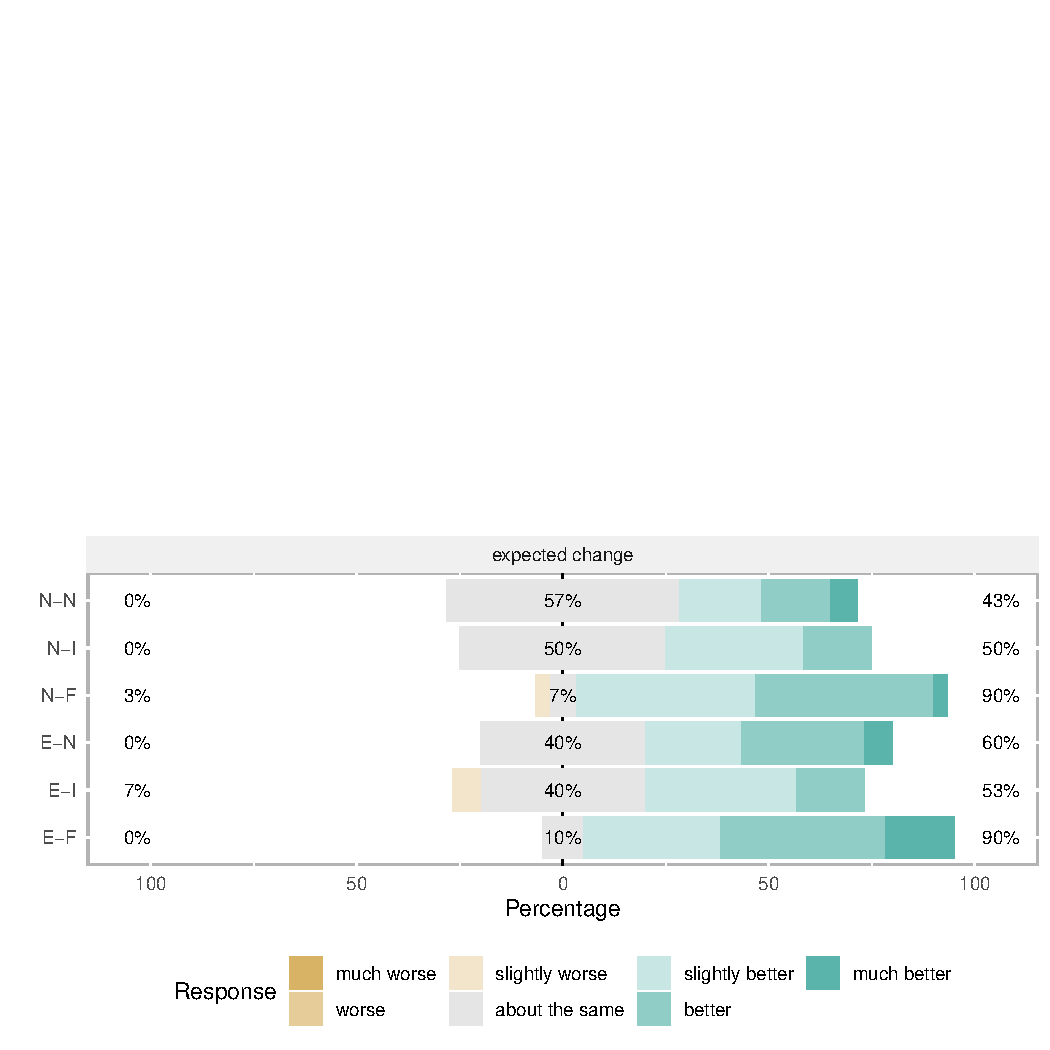
\includegraphics[width=.48\textwidth]{figures/exp-plots-study2.pdf}
    \caption{Study 2 responses for the expected change measure by condition, showing that in general participants expected improvements (green bars), but more in feature-level feedback conditions (E-F and N-F). (See Figure~\ref{fig:study1measures} for a description of y-axis labels).}
    \label{fig:study2exp}
    \vspace{-10pt}
\end{figure}
}
\FigureHighMeasure

\subsection{Results}
Figure~\ref{fig:study2measures} and \ref{fig:study2exp} show the rating responses for the seven main subjective measures by condition.
% satisfaction
Overall, participants were less frustrated with the high quality model than the low quality one (Figure~\ref{fig:study1measures}). 
%
The interaction between explanation and feedback was significant for other subjective measures: trust and acceptance. 
% expected improvement & feedback ability
As in Study~1, feedback impacted expected change but explanation did not, and participants expected the model to improve and wanted the ability to provide feedback.

Regarding task difficulty, participants again performed well: 92\% of their 3,600 answers to us were correct, while 7\% were ``not sure'' and only 1\% were incorrect. 
%
We provide detailed results regarding satisfaction, expectations and perceptions, and quality and desire for feedback in the following sections.


\subsubsection{User Satisfaction}
%
Overall, frustration was lower ($M=2.64$ of 7, $SD=1.54$) compared to the low quality model in Study 1 ($M=3.90$, $SD=1.85$). Perhaps accordingly, there were no significant main or interaction effects on frustration. Open-ended responses suggest explanations exposed the high quality model's \textit{good} behavior.
%
Trust and acceptance ratings were also relatively high compared to Study 1: 5.1 out of 7 on average for trust ($SD=1.5$) and 5.4 for acceptance ($SD=1.5$) here compared to 4.1 for trust ($SD=1.7$) and 4.3 for acceptance ($SD=1.9$) in Study 1. The interaction between explanations and feedback on these measures was significant.

\textbf{Trust and acceptance were affected by the combination of explanations and feedback}.
%
Neither explanation nor feedback had a clear effect on trust; the main effects of \textit{Feedback} ($F_{2,174}=2.59, p=.078$) and \textit{Explanation} ($F_{1,174}=2.00, p=.159$) were not significant. However, the interaction between \textit{Explanation} and \textit{Feedback} was significant ($F_{2,174}=5.69, p=.004$), meaning that certain combinations of explanations and feedback impact trust. 

From the responses (Figure~\ref{fig:study2measures}), when feature-level feedback is requested, not providing an explanation might decrease trust (N-N compared to N-F). And, without feedback, explanation might decrease trust (N-N compared to E-N). After a Holm-Bonferroni correction, only the former posthoc pairwise comparison was significant: participants trusted the model more with neither feedback nor explanation compared to a model with feedback but no explanation ($p < .05$). 

Acceptance shows a similar pattern: while there is no clear effect of either explanation or feedback, some combinations do; the \textit{Explanation} $\times$ \textit{Feedback} interaction was significant ($F_{2,174}=4.11, p=.018$), while the main effects of \textit{Feedback} ($F_{2,174}=1.23, p=.295$) and \textit{Explanation} ($F_{1,174}=.036, p=.850$) were not. While Figure~\ref{fig:study2measures} shows similar trends for acceptance as for trust, no posthoc pairwise comparisons were significant after a Bonferroni correction, so further work is needed to explore this relationship.

\FigureHighExp


% why frustrated
\textbf{Explanations may have shown participants that the model was behaving properly.}
%
Participants gave lower frustration ratings than in Study~1 (Figure~\ref{fig:study2exp}); users said the model was ``good enough'' (49\% of all participants) or would ``save time'' (23\%). Only 15\% of participants felt the model was ``not good enough'', that is, not of an acceptable accuracy for the task. 

In Study~1, explanations exposed issues with the model's highlighted words, resulting in 81\% of the 89 participants who had received explanations in that study thinking the model was ``not good enough.'' Study~2 responses were the opposite: 80\% (of 90) participants who saw explanations thought the model was ``good enough'', and  explicitly described good model behavior, such as \textit{``\dots I was able to see the reasoning from the machine and I agreed with it most of the time''} (HP139, E-F). For Study~2 participants who did not see explanations, only 65\% (of 90) felt the model was ``good enough'', emphasizing how explanations can improve perceptions of model quality with a higher quality model. 

% I think the below is interesting, but we already have a TON of results
%Some of the responses expose differences in what participants consider to be an acceptable accuracy, particularly as it relates to frustration. For example, HP17 (N-F) gave a low frustration rating and said, \textit{``I think it does a really good job. 90ish percent is great,''} whereas HP71 (E-N) said he or she would be frustrated, \textit{``because it wasn't 100\% correct.''} HP5 (E-N) said, \textit{``[...] if I were going to trust this model to the point where I was responsible for what it was doing, I would want almost perfect accuracy [...] I wouldn't be frustrated, though.''} These responses provide some intuition into why \textit{Explanation} and \textit{Feedback} did not impact frustration scores for the high quality model.

\subsubsection{User Expectations for and Perceptions of the Model}
% four points: expected improvement, why, perceived accuracy and perceived understanding
Figure~\ref{fig:study2measures} and \ref{fig:study2exp} show responses for subjective rating scales regarding expectations and perceptions of the model. On average, participants expected improvement ($M=5.0$, $SD=1.0$), thought they understood the model ($M=5.5$, $SD=1.2$), and thought it worked well ($M=5.9$, $SD=.76$).

As detailed below, feature-level feedback caused participants to think the model would improve, and explanation yielded higher perceived understanding. Neither explanation nor feedback had an impact on perceived accuracy. Open-ended responses suggest misconceptions regarding how ML models evolve, providing further explanation for why a substantial portion of participants, regardless of condition, expected the model to improve (Figure~\ref{fig:study2exp}).\footnote{We do not report on participants' simulated model predictions due to space and because trends are in line with the rating data.}  

\textbf{Feature-level feedback increased expected improvement}.
%
As in Study~1, \textit{Feedback} significantly impacted expected change ($F_{2,174}=15.84, p < .001$). Posthoc pairwise comparisons showed that feature-level feedback resulted in higher expected improvement than instance feedback or none (both comparisons $p<.05$). \textit{Explanation} did not have a significant impact on expected change ($F_{1,174}=.79, p=.375$) nor did the \textit{Explanation} $\times$ \textit{Feedback} interaction ($F_{2,174}=1.41, p=.246$).

%\textbf{Participants may still expect correction, but less so when the model is higher quality}.
%
%\lkf{this para really really needs some descriptive stats... in general, one limitation of your results section currently is that it's mostly about p values and descriptives (that people can actually understand) are not mentioned much and instead people have to read the graphs... this example here is perhaps one of the more obvious ones that needs to be fixed though}
%Table~\ref{tab:study2eval} shows the percentage of participants who thought the model would correctly label a previously incorrect email in the evaluation phase.

%\begin{table}[t]
%    \centering
%        \begin{tabular}{cccc}
%    \toprule
%              & \multicolumn{3}{c}{{\bf Feedback}} \\
%              \cline{2-4}
%        {\bf Explanation} & None & Instance & Feature \\
%         \midrule
%        Without & 50\% & 53\% & 57\% \\
%        With &47\% & 57\% & 80\% \\
%        \bottomrule
%    \end{tabular}
%    \caption{Percentage of Study 2 participants ($N=180$) in the different conditions who thought the model would correctly label a previously incorrectly labeled email. Those who did not provide feedback, therefore, thought the model would self correct.}
%    \label{tab:study2eval}
%\end{table}

% why expectations?
\textbf{Participants described misconceptions for how ML changes over time}.
%
Participants gave similar reasons for expecting model change as in Study~1. 27\% of all participants credited the ``feedback'' they provided while 19\% suggested the model was ``self learning.'' Many participants noted similar misconceptions, including, \textit{``my understanding is these sorts of things just get better at what they do the more they do them''} (HP84, E-N) and,
%\textit{``The model is programmed to automatically update its system with corrections and new information''} (HP111, N-N),
 \textit{``it learns with each new experience, and I choose the word `experience' intentionally as the machine gains consciousness''} (HP62, N-I).

% can maybe cut the below, but I do come back to it in the discussion..
Similar to Study~1, 21 (12\%) participants thought their feedback was ``inadequate'' (whether in quality or quantity). Of these, 17 provided instance-level feedback (compared to three who provided no feedback and three who provided feature-level feedback), and suggested that they would have preferred to tell the model \textit{why} it was wrong. 
%HP3 (N-I) said, \textit{``I'm not really sure that it learned anything because of the fact that I didn't explain why it was wrong}, %Maybe it can, but I don't really think so''
For example, HP128 (E-I) said, \textit{``simply telling it that it was wrong may make it less accurate, but it is unlikely to make it more accurate without knowing how it made its mistake.''}

% perceived understanding
\textbf{Explanations increased perceived understanding}.
%
\textit{Explanation} significantly impacted perceived understanding ($F_{1,174}=3.92, p-0.49$). Participants thought they understood the model more when given an explanation (Figure~\ref{fig:study2measures}). Neither the main effect of \textit{Feedback} ($F_{2,174}=.13, p=.876$) nor the \textit{Explanation} $\times$ \textit{Feedback} interaction effect were significant ($F_{2,174}=.53, p=.591$).

\subsubsection{Quality and Desire for User Feedback}
Like in Study~1, participants wanted the ability to provide feedback ($M=6.3$ of 7, $SD=1.0$), regardless of condition (Figure~\ref{fig:study2measures}). There were no significant main or interaction effects on this measure. But how useful is their feedback for the high quality model?

% improvement from feedback
\textbf{Feedback provided only minor improvement}.
%
%Incorporating the Study 2 feedback into the initial, high quality model, resulted in $60$ feature updated models and $60$ instance updated models. 
We incorporated participant's feature-level and instance-level feedback into the model.
While the updated models in Study~1 greatly improved, in Study~2 they did not. The feature updated models averaged 95.8\% accuracy ($SD=.8\%$), only a 1.4 percentage point improvement over the initial high quality model.
The instance updated models had 95.1\% accuracy ($SD=.5\%$; a .7 percentage point improvement). As in Study~1, instance and feature model improvements were similar regardless of whether the participants saw an explanation (difference in accuracy $<.2$).

% feature-level feedback model agreement
\textbf{Participants agreed more with the high quality model's words}.
%
Participants provided 3,589 words as feature-level feedback. Participants were similarly likely to provide new words~(1,942) as reuse model words~(1,647), unlike Study~1 participants who reused less than 25\% of the model's words. 
The 30 participants shown explanations reused provided words (51.6\% overlap of their words to the model's important words), more than the 30 who did not see explanations~(40.2\%). %We saw the opposite effect in Study~1 (there participants used less model words but more when given explanations).

\subsection{Summary}
%
Neither feedback nor explanation impacted frustration, which was generally lower than in Study~1.
For other user experience measures, there were no main effects either, although significant interaction effects on trust and acceptance suggest nuance in how explanations and feedback impact each other.
%
As with the low quality model, feature feedback significantly increased expected change, this time over both instance and no feedback (confirming partial support for \textbf{H2.1}), but explanation did not have an effect. Again, participants generally thought the model would improve. 


%Overall, frustration was lower ($M=2.64$, $SD=1.54$) compared to the low quality model ($M=3.90$, $SD=1.85$). 
%feature-level feedback without explanation significantly reduced trust in the model compared to simply having no explanation and no feedback. We find some evidence that trust decreases when explanations are provided without support for feedback\lkf{please don't add more stats in the summary and discussion... here we are supposed to be making things super easy to read and highlighting the interesting takeaways} ($M=4.97$, $SD=1.77$) compared to no explanations without feedback ($M=5.83$, $SD=1.21$). Further work is needed to explore these interactions. 

%: 48\% of the 60 who did not provide feedback and 62\% of the 120 who provided feedback thought the model would get a previously incorrect email correct. 

%We find some evidence that trust decreases when explanations are provided without support for feedback ($M=4.97$, $SD=1.77$) compared to no explanations without feedback ($M=5.83$, $SD=1.21$).